\documentclass[10pt]{report}
\usepackage{/Users/bradenhoagland/latex/math}

\lhead{Braden Hoagland}
\chead{HW 11}
\rhead{}

\renewcommand{\theenumi}{\alph{enumi}}

\begin{document}
%\tableofcontents

\begin{exer}[7.6: 1]
Find the total Guassian curvature.
\end{exer}
\begin{enumerate}
	\item The ellipsoid is diffeomorphic to the sphere, so $\chi(M)=2$, so by Gauss-Bonnet, so its total Gaussian curvature is $4\pi$.
	\item The surface in Fig. 4.8 has 4 handles, so by Theorem 6.8, $\chi(M)=\chi(\Sigma(h))=\chi(\Sigma)-2h$ = 2-2h=-6. Thus the total Guassian curvatureis $-12\pi$.
	\item $M$ has no handles, so it is diffeomorphic to $\Sigma$, so we have the same situation as in part (a). Thus the total Guassian curvature is $4\pi$.
\end{enumerate}

\begin{exer}[7.6:5]
Show the given change in polygonal decomposition doesn't change the Euler characteristic.
\end{exer}
\begin{enumerate}
	\item We gain no vertices, we get an extra edge, and we get an extra face, so $v-(e+1)+(f+1)=v-e+f$.
	\item We gain a vertex, we gain 3 edges, and we gain 2 faces, so $(v+1)-(e+3)+(f+2)=v-e+f$.
	\item If we start with an $n$-gon, then we'll gain one vertex, we'll gain $n$ edges, and we'll gain $n-1$ faces, so $(v+1)-(e+n)+(f+n-1)=v-e+f$.
\end{enumerate}

\pagebreak
\begin{exer}[7.6: 7]
Check Gauss-Bonnet formula for restriction of geographical patch on sphere to $0 \leq u,v \leq \pi/4$.
\end{exer}
Since $K$ is constant on $\Sigma$, the total Gaussian curvature is just $K=1/r^2$ times the area of the region. We can manually compute the area form to be ${\Vert{\mathbf{x}_{u}\times \mathbf{x}_{v}}\Vert} = r^2\cos v\;du\;dv$, so we have
\[
\int_{} \int_{R} K\;dM = \frac{1}{r^2} \int_{0}^{\pi/4} \int_{0}^{\pi/4} r^2 \cos v\;du\;dv = \frac{\sqrt{2} \pi}{8} .
\] 
The only non-geodesic boundary curve on our region is the top curve $\alpha$ (the two vertical lines are lines of longitude and the bottom curve is the equator), so their geodesic curvature is 0. To calculate the total geodesic curvature of the $\alpha$, we note that it is symmetric about the center of the sphere. Then if $\phi$ is an angle function from $\alpha'$ to $E_1$, $\phi$ will be the same when evaluated at any two points on $\alpha$. Thus by Lemma 6.2,
\[
	\int_{\alpha} \kappa_{g}\;ds = \varphi(b) -\varphi(a) + \int_{\alpha} \omega_{12} =  \int_{\alpha} \omega_{12}.
\] 
From \S 7.3 Example 3.7, we get that the connection form on the geographical patch is $\omega_{12}=\sin \;du$. After noting that the orientation of $\alpha$ is reversed, this becomes
\[
	\int_{\alpha} \kappa_{g}\;ds = - \int_{0}^{\pi/4} \sin \left( \frac{\pi}{4}  \right)\;du = -\int_{0}^{\pi/4} \frac{\sqrt{2} }{2} \;du = -\frac{\sqrt{2} }{8} \pi.
\] Finally, we note that since each of our boundary curves is perpendicular to the other two that it meets at the corners of our region, each exterior angle is $\pi/2$, so
\[
\sum \varepsilon_{i} = 2\pi.
\] Putting it all together, we get
\[
\int_{} \int_{R} K\;dM + \int_{\alpha} \kappa_{g}\;ds + \sum \varepsilon_{i} = \frac{\sqrt{2} \pi}{8} - \frac{\sqrt{2} \pi}{8} + 2\pi = 2\pi,
\] as indicated by the Gauss-Bonnet formula.

\pagebreak
\begin{exer}[7.6: 8]
	The degree of the Gauss map of a compact oriented surface in $\mathbb{R}^{3}$ is $\chi(M)/2$.
\end{exer}
Gauss-Bonnet gives
\[
	2\pi\chi(M) = \int_{} \int_{M} K\;dM.
\] And by \S 6.8 Corollary 8.5, the total Gaussian curvature of an oriented surface equals the algebraic area of the image of its Gauss map. Thus the algebraic area of $G(M)$ is $2\pi\chi(M)$.

Since the total area of $\Sigma$ is $4\pi$, the degree of $G$ is
\[
	\frac{\text{algebraic area of } G(M)}{\text{area of } \Sigma} = \frac{2\pi\chi(M)}{4\pi} = \frac{\chi(M)}{2} .
\] 

\begin{exer}[7.6: 9]
Can you decompose a sphere into hexagons? A torus?
\end{exer}
\textbf{Sphere:} No. Each vertex lies at the intersection of 3 faces, so for all 6 vertices per hexagon, we count each of them 3 times. Thus the total number of vertices is $v = 6f/3 = 2f$. Similarly, each edge lies at the intersection of 2 faces, so $e = 6f/2 = 3f$. Then
\[
	\chi(M) = v-e+f = 2f-3f+f = 0.
\] But $\chi(\Sigma)=2 \neq 0$, so since the Euler characteristic is preserved by diffeomorphisms, the sphere cannot be tiled by hexagons.

\textbf{Torus:} Yes. Consider the tiling below.
\begin{figure}[H]
	\centering
	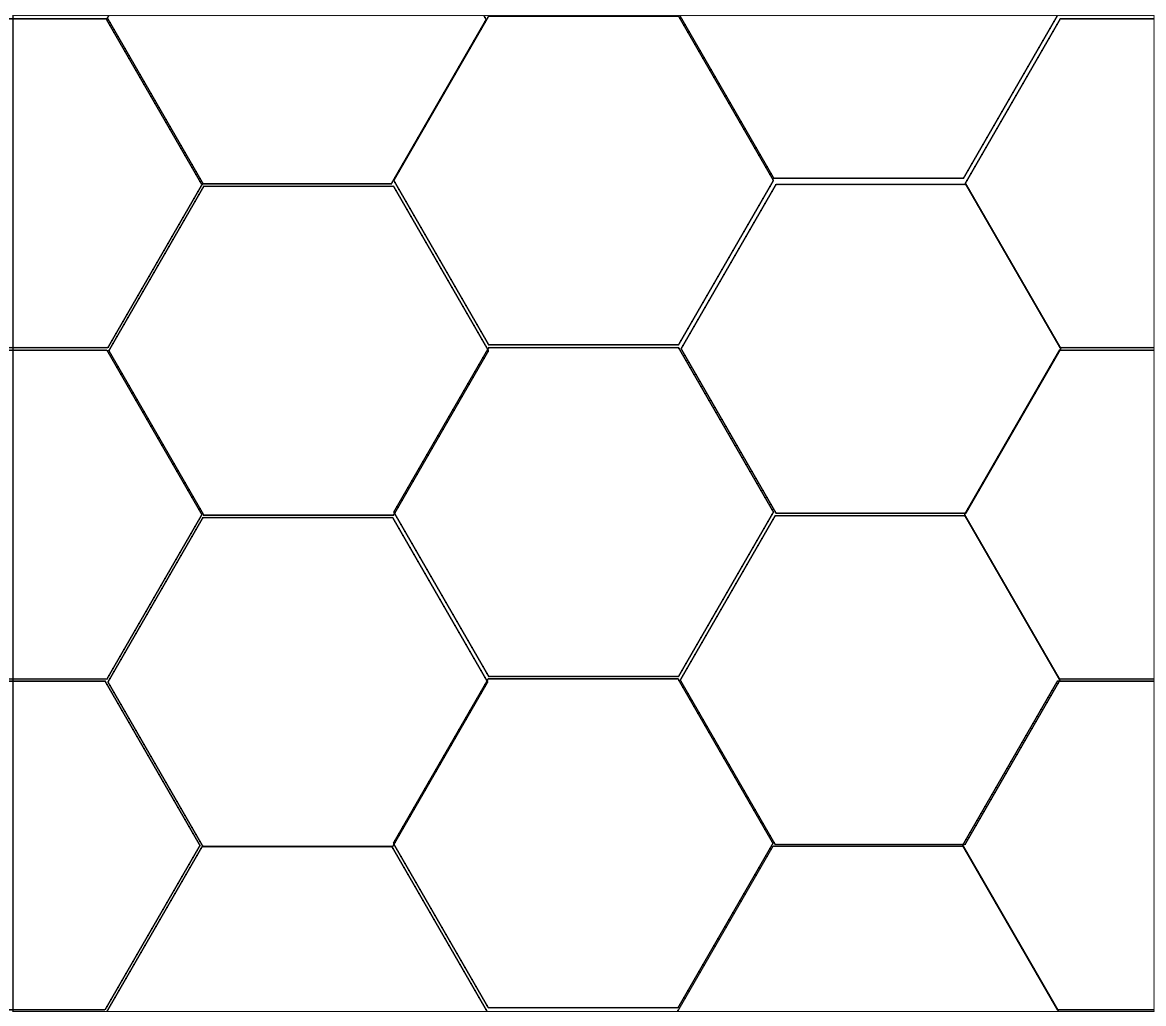
\includegraphics[scale=0.2]{fig/torus}
\end{figure}
After identifying opposite edges with the same orientation, we get a torus with a hexagonal tiling.


\pagebreak
\begin{exer}[7.7: 2]
Show that there are no geodesic $n$-polygons on surfaces with $K \leq 0$.
\end{exer}
Polygons have Euler characteristic 1, so by Theorem 7.5 (after noting that $\kappa_{g}=0$ since our boundary curves are geodesics),
\[
	\int_{} \int_{\mathscr{P}} K\;dM + \sum_{i=1}^{n} \varepsilon_{j}= 2\pi\chi(\mathscr{P}) = 2\pi.
\] 
When $n=0$, we get that the total Gaussian curvature is $2\pi$. But this is impossible, since $K \leq 0$ implies that the total Gaussian curvature is non-positive.

When $n=1$, we have $\int_{} \int_{\mathscr{P}} K\;dM + \varepsilon_1=2\pi$. Since $K \leq 0$, this implies $\varepsilon_1 \geq 2\pi$. But this is also impossible, as turning $2\pi$ would mean that the curve turns back onto itself.

When $n=2$, we similarly have $\varepsilon_1 + \varepsilon_2 \geq 2\pi$. But this also implies that the curve would have to turn back onto itself, so this is also impossible.

\pagebreak
\begin{exer}[]
Describe the Gaussian curvature of a smoothed tetrahedron and smoothed cube.
\end{exer}
First we note that both surfaces are diffeomorphic to the sphere, so $\chi(M)=2$ for both. Then by Gauss-Bonnet,
\[
	\int_{} \int_{M} K\;dM = 2\pi\chi(M) = 4\pi
\] for both surfaces. Because both surfaces are symmetric, we expect each symmetric region to contribute the same amount to this $4\pi$. Furthermore, we claim that the only contributions to the Gaussian curvature come from the regions surrounding the smoothed over vertices.

Note that since the face regions (where no smoothing occurred) are flat on both surfaces, so the Gaussian curvature there is necessarily 0. To describe $K$ around the edge and vertex regions, we can use \S 6.8 Corollary 8.5, which says that the total Gaussian curvature of a small region is the same as the area of that region's image under the Gauss map.

Then for some point along an edge, the image of the Gauss map traces out a line. Since lines have 0 area on the sphere (see the picture below), this means that small regions around a point on an edge don't contribute to the total Gaussian curvature, so $K=0$ in the edge regions.

\begin{figure}[H]
	\centering
	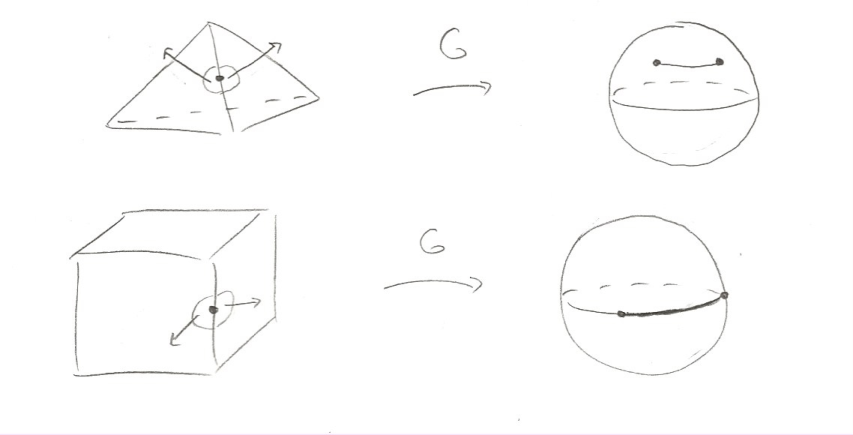
\includegraphics[scale=0.8]{fig/edge.pdf}
\end{figure}


For small regions around a vertex point, the image under the Gauss map has nontrivial area (see the picture below). Thus the vertex regions contribute to the total Gaussian curvature, so $K$ is nonzero in these regions.

\begin{figure}[H]
	\centering
	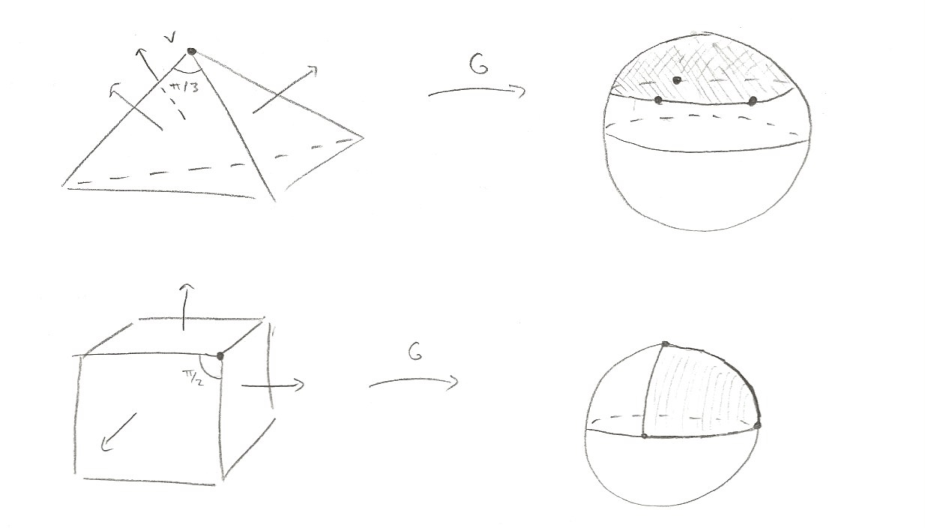
\includegraphics[scale=0.6]{fig/vertex.pdf}
\end{figure}


To find the contribution from each vertex point, we can use deficit angles. Suppose $\iota_i$ is an interior angle at a vertex, then the corresponding exterior angle is $\varepsilon_i = \pi-\iota_i$. We know that the total Gaussian curvature of this region is the deficit angle
\[
	\int_{} \int_{\mathscr{R}} K\;dM = 2\pi - \sum_i \iota_i.
\] Thus for the tetrahedron, since $\iota_i = \pi/3$ and each vertex has three $\iota_i$, each vertex contributes
\[
	2\pi - \pi = \pi
\] total Gaussian curvature. As a sanity check, since we have 4 vertices, the total Gaussian curvature over the whole surface comes out to $4\pi$. For the cube, since $\iota_i = \pi/2$ and each vertex has three $\iota_i$, each vertex contributes
\[
2\pi-3\pi/2 = \pi/2
\] total Gaussian curvature. Since we have eight vertices total, there is then $4\pi$ total Gaussian curvature over the whole surface, as expected.

As a final note, the specific function $K$ will depend on how much the tetrahedron/cube are smoothed. If we smooth more, then $|K|$ will decrease at all points but become nonzero at more points, essentially spreading out around the vertex regions. If there is very little smoothing, then $K$ will be sharply concentrated near the vertices.

\end{document}
